\documentclass{report}\usepackage[]{graphicx}\usepackage[]{color}
%% maxwidth is the original width if it is less than linewidth
%% otherwise use linewidth (to make sure the graphics do not exceed the margin)
\makeatletter
\def\maxwidth{ %
  \ifdim\Gin@nat@width>\linewidth
    \linewidth
  \else
    \Gin@nat@width
  \fi
}
\makeatother

\definecolor{fgcolor}{rgb}{0.345, 0.345, 0.345}
\newcommand{\hlnum}[1]{\textcolor[rgb]{0.686,0.059,0.569}{#1}}%
\newcommand{\hlstr}[1]{\textcolor[rgb]{0.192,0.494,0.8}{#1}}%
\newcommand{\hlcom}[1]{\textcolor[rgb]{0.678,0.584,0.686}{\textit{#1}}}%
\newcommand{\hlopt}[1]{\textcolor[rgb]{0,0,0}{#1}}%
\newcommand{\hlstd}[1]{\textcolor[rgb]{0.345,0.345,0.345}{#1}}%
\newcommand{\hlkwa}[1]{\textcolor[rgb]{0.161,0.373,0.58}{\textbf{#1}}}%
\newcommand{\hlkwb}[1]{\textcolor[rgb]{0.69,0.353,0.396}{#1}}%
\newcommand{\hlkwc}[1]{\textcolor[rgb]{0.333,0.667,0.333}{#1}}%
\newcommand{\hlkwd}[1]{\textcolor[rgb]{0.737,0.353,0.396}{\textbf{#1}}}%
\let\hlipl\hlkwb

\usepackage{framed}
\makeatletter
\newenvironment{kframe}{%
 \def\at@end@of@kframe{}%
 \ifinner\ifhmode%
  \def\at@end@of@kframe{\end{minipage}}%
  \begin{minipage}{\columnwidth}%
 \fi\fi%
 \def\FrameCommand##1{\hskip\@totalleftmargin \hskip-\fboxsep
 \colorbox{shadecolor}{##1}\hskip-\fboxsep
     % There is no \\@totalrightmargin, so:
     \hskip-\linewidth \hskip-\@totalleftmargin \hskip\columnwidth}%
 \MakeFramed {\advance\hsize-\width
   \@totalleftmargin\z@ \linewidth\hsize
   \@setminipage}}%
 {\par\unskip\endMakeFramed%
 \at@end@of@kframe}
\makeatother

\definecolor{shadecolor}{rgb}{.97, .97, .97}
\definecolor{messagecolor}{rgb}{0, 0, 0}
\definecolor{warningcolor}{rgb}{1, 0, 1}
\definecolor{errorcolor}{rgb}{1, 0, 0}
\newenvironment{knitrout}{}{} % an empty environment to be redefined in TeX

\usepackage{alltt}
\usepackage{mparhack}
\usepackage{xstring}
\usepackage{color}
\usepackage{multicol}
\usepackage[landscape,margin=.25in,bottom=-.35in,includehead,includefoot]{geometry}

\pagestyle{empty}



\newcommand{\asection}[1]{{\sf\bfseries #1}}
\renewenvironment{knitrout}{\vspace*{-.1in}}{\vspace*{-.1in}} % an empty environment to be redefined in TeX
\IfFileExists{upquote.sty}{\usepackage{upquote}}{}
\begin{document}
\parindent=0pt

\vspace*{-.85in}\begin{center}
{\sf \bfseries \Large Enough R for Data Computing Fundamentals}\\
\texttt{dtkaplan.github.io/comp110/DCF-materials-book/Handouts/EnoughDCF.pdf}
\end{center}

\def\opt#1{#1}
\def\squeeze{\vspace*{-4ex}}

\begin{multicols}{4}
\raggedright

\small
\asection{Getting Started} Load the package whenever you start a new session.

\begin{knitrout}
\definecolor{shadecolor}{rgb}{0.969, 0.969, 0.969}\color{fgcolor}\begin{kframe}
\begin{alltt}
\hlkwd{library}\hlstd{(DataComputing)}
\end{alltt}
\end{kframe}
\end{knitrout}
Don't have DataComputing?  Install the package:
\begin{knitrout}
\definecolor{shadecolor}{rgb}{0.969, 0.969, 0.969}\color{fgcolor}\begin{kframe}
\begin{alltt}
\hlstd{devtools}\hlopt{::}\hlkwd{install_github}\hlstd{(}
  \hlstr{"DataComputing/DataComputing"}\hlstd{)}
\end{alltt}
\end{kframe}
\end{knitrout}

\smallskip

\asection{Overview} The data verbs, summary functions, and transformation functions enable you to transfigure data into a glyph- or analysis-ready form.

\smallskip

The basic syntax:
\begin{knitrout}
\definecolor{shadecolor}{rgb}{0.969, 0.969, 0.969}\color{fgcolor}\begin{kframe}
\begin{alltt}
Result <-
  DT %>% 
  \hlkwd{verb1}( [some args] ) %>%
  \hlkwd{verb2}( [more args] ) %>%
  ... and so on as needed ...
\end{alltt}
\end{kframe}
\end{knitrout}

$\bullet$ \texttt{<-} is the assignment symbol.
\smallskip

$\bullet$ \texttt{\%>\%} is the chaining symbol: take the output of the left expression and make it the input of the right expression.

\smallskip

$\bullet$ Lines that {\bf end} with \texttt{<-} or \texttt{\%>\%} identify that the next line continues the expression. 

\medskip

\asection{Data Tables} are organized into cases and variables.  Variables are either quantitative or categorical: numbers or words. Two examples used here:


\smallskip

\begin{small}
$\bullet$ First example data table: \texttt{DT}
\begin{knitrout}
\definecolor{shadecolor}{rgb}{0.969, 0.969, 0.969}\color{fgcolor}\begin{kframe}
\begin{verbatim}
##     name sex height weight
## 1   Alma   F   1.64     54
## 2 Junior   M   1.82     73
## 3   Gary   M   1.71     64
## 4 Kristy   F   1.75     61
\end{verbatim}
\end{kframe}
\end{knitrout}
\texttt{sex} is categorical, \texttt{height} and \texttt{weight} are quantitative.

\smallskip

$\bullet$ Second example data table: \texttt{Sports}

\begin{knitrout}
\definecolor{shadecolor}{rgb}{0.969, 0.969, 0.969}\color{fgcolor}\begin{kframe}
\begin{verbatim}
##   name      sport
## 1 Fred   Football
## 2 Alma Water Polo
## 3 Alma     Hockey
## 4 Gary   Football
\end{verbatim}
\end{kframe}
\end{knitrout}
\end{small}


\smallskip

\asection{Quick presentation of data tables}

\begin{knitrout}
\definecolor{shadecolor}{rgb}{0.969, 0.969, 0.969}\color{fgcolor}\begin{kframe}
\begin{alltt}
\hlkwd{str}(DT)  \hlkwd{summary}(DT)  
\hlkwd{nrow}(DT) \hlkwd{names}(DT)
\hlkwd{head}(DT) \hlkwd{tail}(DT) \hlkwd{View}(DT)
\end{alltt}
\end{kframe}
\end{knitrout}

\vfill
\columnbreak

\definecolor{light-gray}{gray}{0.97}

\hspace*{-.18in}\colorbox{light-gray}{\parbox{5.35in}{\normalsize\hspace*{.2in}\asection{Data Verbs} take a data table as input and return as output a modified table.

\smallskip

\begin{tabular}{llrl}
Verb & Task & Argument(s) & Example\\\hline
\texttt{filter()} & Winnow cases & Comparison & \texttt{filter(year$>$2000)}\\
\texttt{mutate()} & Adds vars. & Transformation & \texttt{mutate(bmi=weight/height\^{}2)}\\
\texttt{summarise()} & Combines cases & Summary & \texttt{summarise(ave=mean(height))} \\
\texttt{select()} & Drops vars. & Var. Names & \texttt{select(sex, height)}\\
\texttt{arrange()} & Order cases & Var. Names & \texttt{arrange(height)}\\
Join & Combines tables & Data Table & See \asection{Various Joins} \\
\texttt{group\_by()} & Split into groups & Var. Names & \texttt{group\_by(sex)}\\\hline
\end{tabular}

\smallskip
All the examples assume a data table is being chained in, e.g. \texttt{DT \%>\% group\_by(sex)}.}}
\bigskip

\asection{Grouping Operations}

\texttt{group\_by()} can be used with several data verbs.

\smallskip
Summarize within each group property
\begin{knitrout}
\definecolor{shadecolor}{rgb}{0.969, 0.969, 0.969}\color{fgcolor}\begin{kframe}
\begin{alltt}
\hlstd{DT} \hlopt \hlkwd{group_by}\hlstd{(sex)} \hlopt
  \hlkwd{summarise}\hlstd{(}\hlkwc{tallest} \hlstd{=} \hlkwd{max}\hlstd{(height))}
\end{alltt}
\end{kframe}
\end{knitrout}

\smallskip
Compare each case to a group property
\begin{knitrout}
\definecolor{shadecolor}{rgb}{0.969, 0.969, 0.969}\color{fgcolor}\begin{kframe}
\begin{alltt}
\hlstd{DT} \hlopt \hlkwd{group_by}\hlstd{(sex)} \hlopt
  \hlkwd{mutate}\hlstd{(}\hlkwc{rel} \hlstd{= height}\hlopt{-}\hlkwd{mean}\hlstd{(height))}
\end{alltt}
\end{kframe}
\end{knitrout}

\smallskip
Choose cases from each group.
\begin{knitrout}
\definecolor{shadecolor}{rgb}{0.969, 0.969, 0.969}\color{fgcolor}\begin{kframe}
\begin{alltt}
\hlstd{DT} \hlopt \hlkwd{group_by}\hlstd{(sex)} \hlopt
  \hlkwd{filter}\hlstd{(}\hlkwd{rank}\hlstd{(height)} \hlopt{==} \hlnum{1}\hlstd{)}
\end{alltt}
\end{kframe}
\end{knitrout}

\smallskip

\asection{Various Joins} differ mainly in how they deal with unmatched cases.

Cases matched with *all* variables that appear in both tables, just \texttt{name} in the example.

$\bullet$ Keep all cases that have a match:\\
\texttt{DT \%>\% inner\_join(Sports)}
\begin{small}
\begin{knitrout}
\definecolor{shadecolor}{rgb}{0.969, 0.969, 0.969}\color{fgcolor}\begin{kframe}
\begin{verbatim}
##   name sex height weight      sport
## 1 Alma   F   1.64     54 Water Polo
## 2 Alma   F   1.64     54     Hockey
## 3 Gary   M   1.71     64   Football
\end{verbatim}
\end{kframe}
\end{knitrout}
\end{small}
Note: output has *both* of Alma's sports.


$\bullet$ Keep all cases from left table:\\
\texttt{DT \%>\% left\_join(Sports)}\\

$\bullet$ Keep unmatched cases:\\
\texttt{DT \%>\% anti\_join( Sports )}



\vfill
\columnbreak
\vspace*{1.75in}

\asection{To Use in Arguments to Data Verbs}

\medskip

\asection{Reduction Functions} take a variable as input and return a single number.

\begin{knitrout}
\definecolor{shadecolor}{rgb}{0.969, 0.969, 0.969}\color{fgcolor}\begin{kframe}
\begin{alltt}
\hlkwd{mean}(height, na.rm = TRUE )
\hlkwd{max}(weight)  \hlkwd{n}()
\hlkwd{min}(weight)  \hlkwd{n_distinct}()
\end{alltt}
\end{kframe}
\end{knitrout}

\medskip
\asection{Transformation Functions}, used with \texttt{mutate()}, take one or more variables as input and return a variable (with the same number of cases).

\begin{knitrout}
\definecolor{shadecolor}{rgb}{0.969, 0.969, 0.969}\color{fgcolor}\begin{kframe}
\begin{alltt}
\hlkwd{rank}\hlstd{(var)}
\hlkwd{pmin}\hlstd{(var1, var2)} \hlcom{#smaller of the two}
\hlstd{var1}\hlopt{/}\hlstd{(var1}\hlopt{+}\hlstd{var2)} \hlcom{#division, addition}
\end{alltt}
\end{kframe}
\end{knitrout}

\smallskip

\asection{Comparison Expressions}

\texttt{filter()} uses one or more comparison expression to determine which cases to pass through.
\begin{knitrout}
\definecolor{shadecolor}{rgb}{0.969, 0.969, 0.969}\color{fgcolor}\begin{kframe}
\begin{alltt}
\hlstd{DT} \hlopt \hlkwd{filter}\hlstd{(height} \hlopt{<} \hlnum{1.8} \hlstd{)}
\hlstd{DT} \hlopt \hlkwd{filter}\hlstd{(name} \hlopt{==} \hlstr{"Junior"} \hlstd{)}
\hlstd{DT} \hlopt \hlkwd{filter}\hlstd{(sex} \hlopt{==} \hlstr{"F"}\hlstd{, height} \hlopt{<} \hlnum{1.8}\hlstd{)}
\hlstd{DT} \hlopt \hlkwd{filter}\hlstd{(count} \hlopt{>}\hlnum{2000}\hlstd{, count} \hlopt{<}\hlnum{10000}\hlstd{)}
\hlstd{DT} \hlopt \hlkwd{filter}\hlstd{(name} \hlopt \hlkwd{c}\hlstd{(}\hlstr{"Alma"}\hlstd{,}\hlstr{"Gary"}\hlstd{))}
\end{alltt}
\end{kframe}
\end{knitrout}

\smallskip

\asection{Variable Names}

\texttt{group\_by()}, \texttt{select()}, and \texttt{arrange()} take one or more variable names as arguments, in addition to the chained in data table.

\smallskip

\asection{Datasets in DataComputing}

Get a listing with \texttt{data(~package="DataComputing"~)}.  All those listed are available by name once the DCF package is loaded.  See also \texttt{mosaicData} and \texttt{NHANES} packages.


\vfill
\columnbreak

\asection{Graphics with ggplot}

$\bullet$ Create a new graphic: \texttt{ggplot()}\\
\smallskip

$\bullet$ Functions to add graphical layers\\
\texttt{geom\_point()}
\texttt{geom\_text()}
\texttt{geom\_bar()}, etc. Others: \texttt{xlab()}, \texttt{ylab}, \texttt{xlim(low,high)}, \texttt{ylim(low,high)}
\smallskip


$\bullet$ \texttt{aes()} to *map* variables to graphical attributes (aesthetics), e.g. Distinguish groups using color \texttt{aes(color=sex, ...)}. *Set* properties to constants outside \texttt{aes()}.

Example:
\begin{knitrout}
\definecolor{shadecolor}{rgb}{0.969, 0.969, 0.969}\color{fgcolor}\begin{kframe}
\begin{alltt}
\hlstd{DT} \hlopt
 \hlkwd{ggplot}\hlstd{(}\hlkwd{aes}\hlstd{(}\hlkwc{x} \hlstd{= height,} \hlkwc{y} \hlstd{= weight))} \hlopt{+}
 \hlkwd{geom_point}\hlstd{(}\hlkwc{size} \hlstd{=} \hlnum{5}\hlstd{,}         \hlcom{#Setting}
            \hlkwd{aes}\hlstd{(}\hlkwc{color}\hlstd{=sex,} \hlkwc{shape}\hlstd{=sex))} \hlopt{+}
 \hlkwd{geom_text}\hlstd{(}\hlkwd{aes}\hlstd{(}\hlkwc{label} \hlstd{= name))}                         \hlopt{+}
                                            \hlkwd{xlim}\hlstd{(}\hlnum{1.63}\hlstd{,}\hlnum{1.85}\hlstd{)} \hlopt{+} \hlkwd{ylim}\hlstd{(}\hlnum{50}\hlstd{,}\hlnum{80}\hlstd{)}
\end{alltt}
\end{kframe}
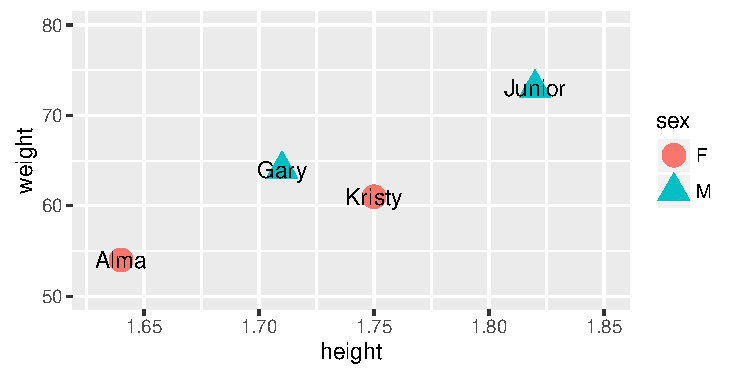
\includegraphics[width=\maxwidth]{figuresunnamed-chunk-18-1} 

\end{knitrout}



\smallskip

\asection{Choropleth Maps}

\texttt{mUSMap()} has a  \texttt{key=} argument identifies the variable naming the geographic entity. \texttt{fill=} specifies the quantity to be plotted.
\begin{knitrout}
\definecolor{shadecolor}{rgb}{0.969, 0.969, 0.969}\color{fgcolor}\begin{kframe}
\begin{alltt}
\hlkwd{mUSMap}\hlstd{(}\hlkwc{data}\hlstd{=StateData,}
            \hlkwc{key}\hlstd{=}\hlstr{"State"}\hlstd{,}\hlkwc{fill}\hlstd{=}\hlstr{"age"}\hlstd{)}
\end{alltt}
\end{kframe}
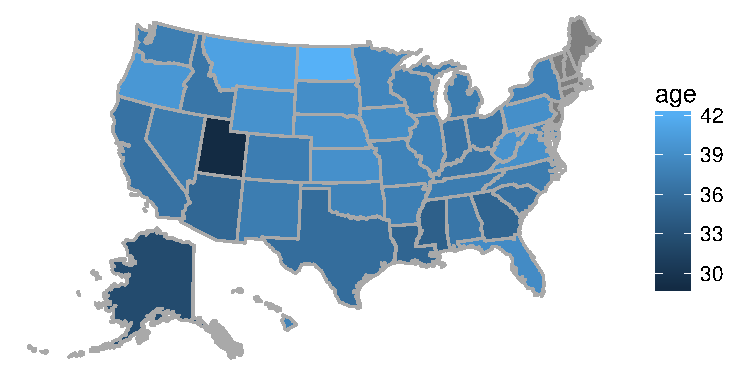
\includegraphics[width=\maxwidth]{figuresunnamed-chunk-20-1} 

\end{knitrout}
\texttt{mWorldMap()} is used in the same way.

\end{multicols}
\end{document}

